%!TEX root = ../dokumentation.tex

\section{Content Modeling}
Der Gestaltungsprozess unter Anwendung verschiedener Techniken der MCI hat zum Ziel, eine Designlösung zu erarbeiten, welche die Gebrauchstauglichkeit eines System im Vergleich zu vorhandenen Optionen steigert. Die vorherigen Kapitel beschrieben die Auseinandersetzung mit vorhandenen Benutzern und ihren zu erledigenden Aufgaben und Strukturen. Im Anschluss an das role model und task model, sieht das Vorgehensmodell die Entwicklung des content models vor.
Hierbei handelt es darum einen ersten Schritt in Richtung Interfacedesign zu machen und den abstrakten Aufbau der gesamten  Interface Architektur zu modellieren. Im Projektverlauf dient dieses Modell dazu den Designprozess zu beschleunigen, indem vorerst die reine Struktur der Interaktion Contexts innerhalb des Systems analysiert wird und darauf aufbauend getestet werden kann, inwiefern die Systemkomponten bisher in Beziehung zueinander stehen.
Anhand des Ergebnisses, lässt sich mit Usern, in unserem Fall im Projektteam, in einem sehr frühen Punkt der Projektphase über den Systementwurf sprechen, indem die reine Struktur fokusiert werden kann. Dieser Vorgang wird auch als Rapid Abstract Prototyping bezeichnet und die anschließende Evaluation sollte dazu dienen, vorherige Ausarbeitungen aus Systemsicht zu evaluieren.

\newpage
\subsection{Abstract Prototype 1}
Nach Vorgehensbeschreibung von Constantine \& Lockwood\footnote{Unter Verwendung von http://www.foruse.com/articles/abstractprototypes.htm und L. Constantine \& L. Lockwood: Software for use, 2003 ab Seite 125}, wurde der erste Prototyp entwickelt. 

\subsubsection{Interaction Contexts }
Auf Basis der essentiell use cases in der ersten Version, wurden die interface contexts erstellt. Jedem use case wurde dabei ein eigener working space gewidmet und anschließend tools und materials bestimmt. Einzelne use cases ließen sich dabei nicht zusammenfassen.
Beispielhaft sind die beiden Interface Contexte in Abbildung \ref{interfaceContents1} dargestellt und zeigen den einfachen Aufbau dieses Prototyps.\footnote{Gesamtes Bilderset im Anhang Teil A}

\begin{figure}[H]
\centering
\hfill
\subfloat[aktionAuswählen \label{pic:aktionAuswaehlen}]{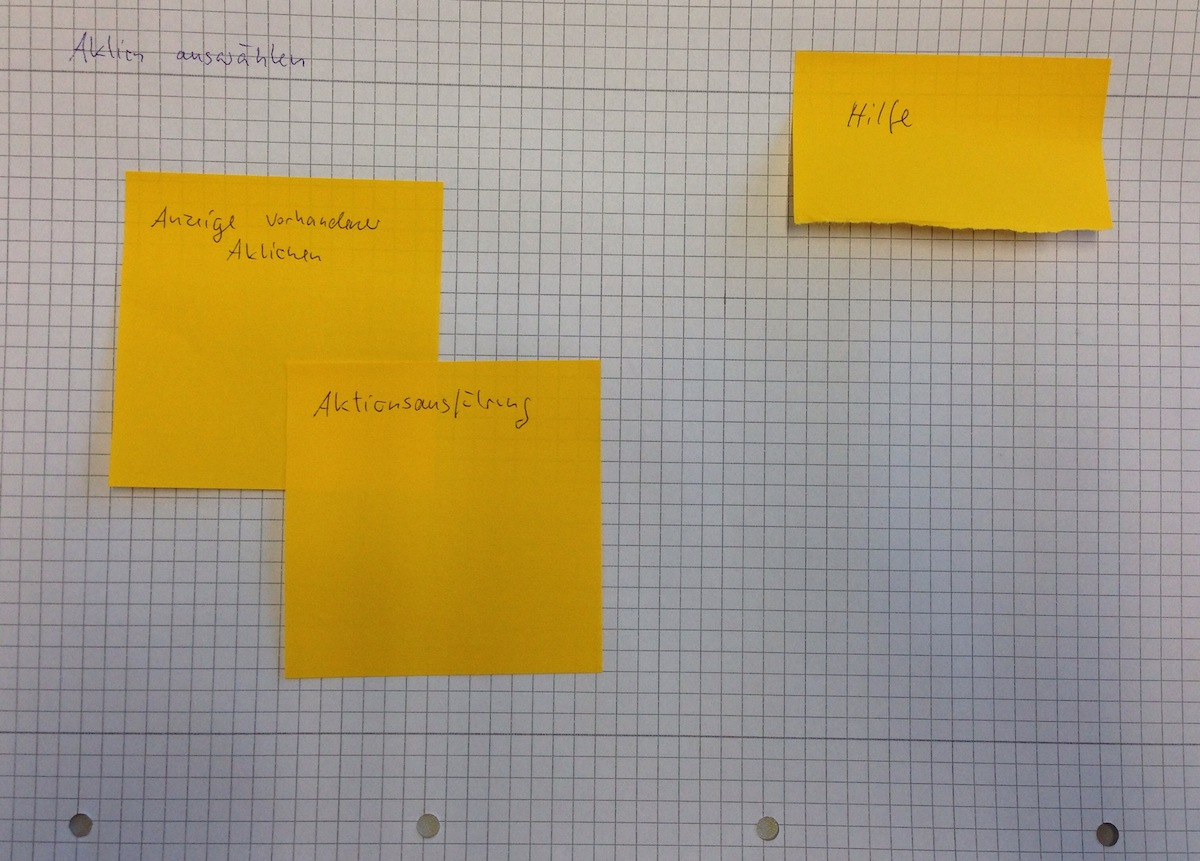
\includegraphics[width=.5\textwidth]{./images/abstract/version1/aktionAuswaehlen.JPG}}
\hfill % alternativ auch \hspace{1cm} für genaue Angaben
\subfloat[sucheMietobjekt \label{pic:sucheMietobjekt}]{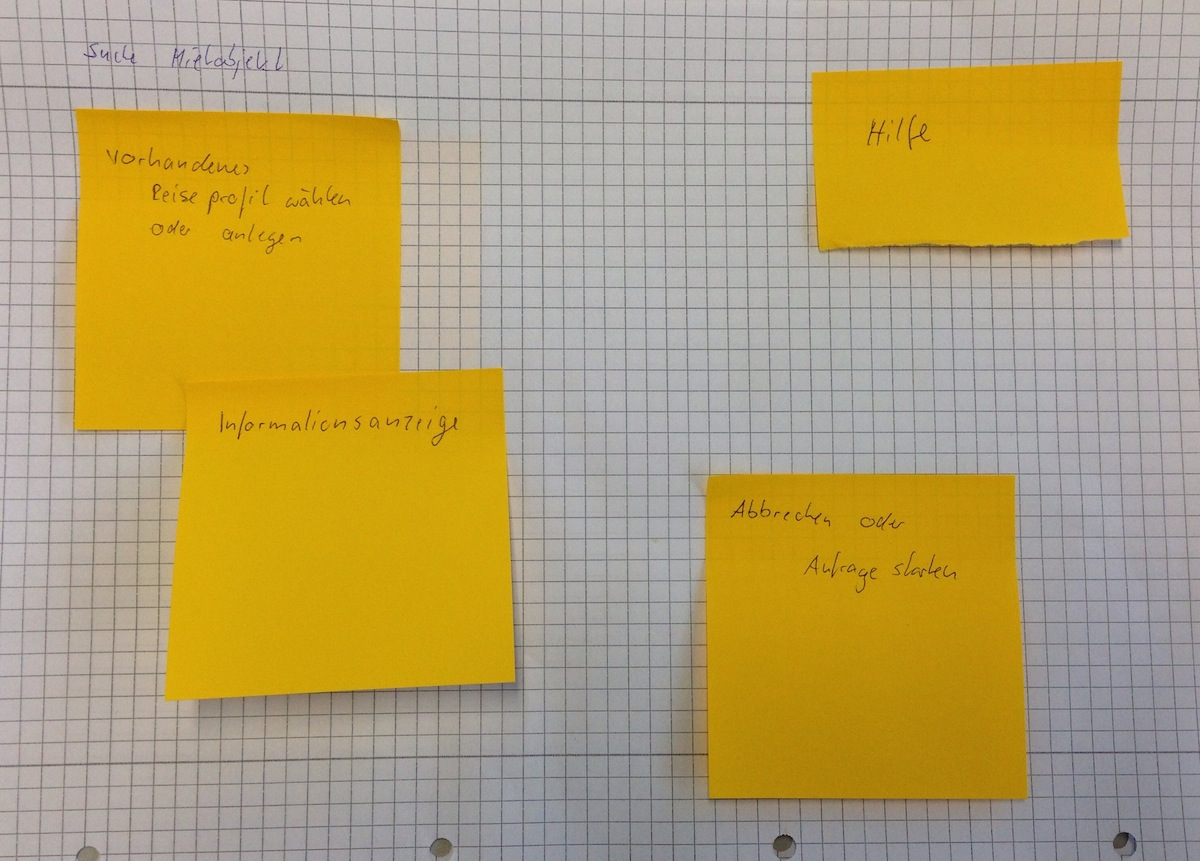
\includegraphics[width=.5\textwidth]{./images/abstract/version1/sucheMietobjekt.JPG}}
\hfill %
\caption{Inter. Context AP1: aktionAuswählen und sucheMietobjekt }
\label{interfaceContents1}
\end{figure}

Während der Ausarbeitung der einzelnen interaction context, machte das allgemeine Verständnis zu tools und materials noch Probleme und das Ausarbeiten auf Grundlage der essential use cases war, zumindest nach eigenen Einschätzungen, nicht immer so konkret, wie es die Entwickler gedenken. Auch das Nachlesen in weiteren Quellen konnte keine komplett sichere Erkenntnis liefern, was die genauen Details des Models angeht. Die entstandenen Modelle basieren daher auf einen Kompromiss aus eigenen Vorstellungen und Vorgaben, wobei das grundlegende Ziel dieser Modellierung klar war.

\newpage
\subsubsection{Context Navigation Map}
Anhand der einzelnen Interface Contexts, wurde die Navigation Map in Abbildung \ref{fig:navigationmap1} entwickelt und verdeutlicht, wie die einzelnen Interfaceseiten konzeptionell zusammenhängen. Diese Grafik beschränkt sich dabei noch auf die Bezeichnung der Kontexte und die einzelnen Aktionen, welche den Kontextwechsel triggern. Eine genauere Darstellung sollte erst in der überarbeiteten Version (Abbildung \ref{interfaceContents2}) erreicht werden.

\begin{figure}[H]
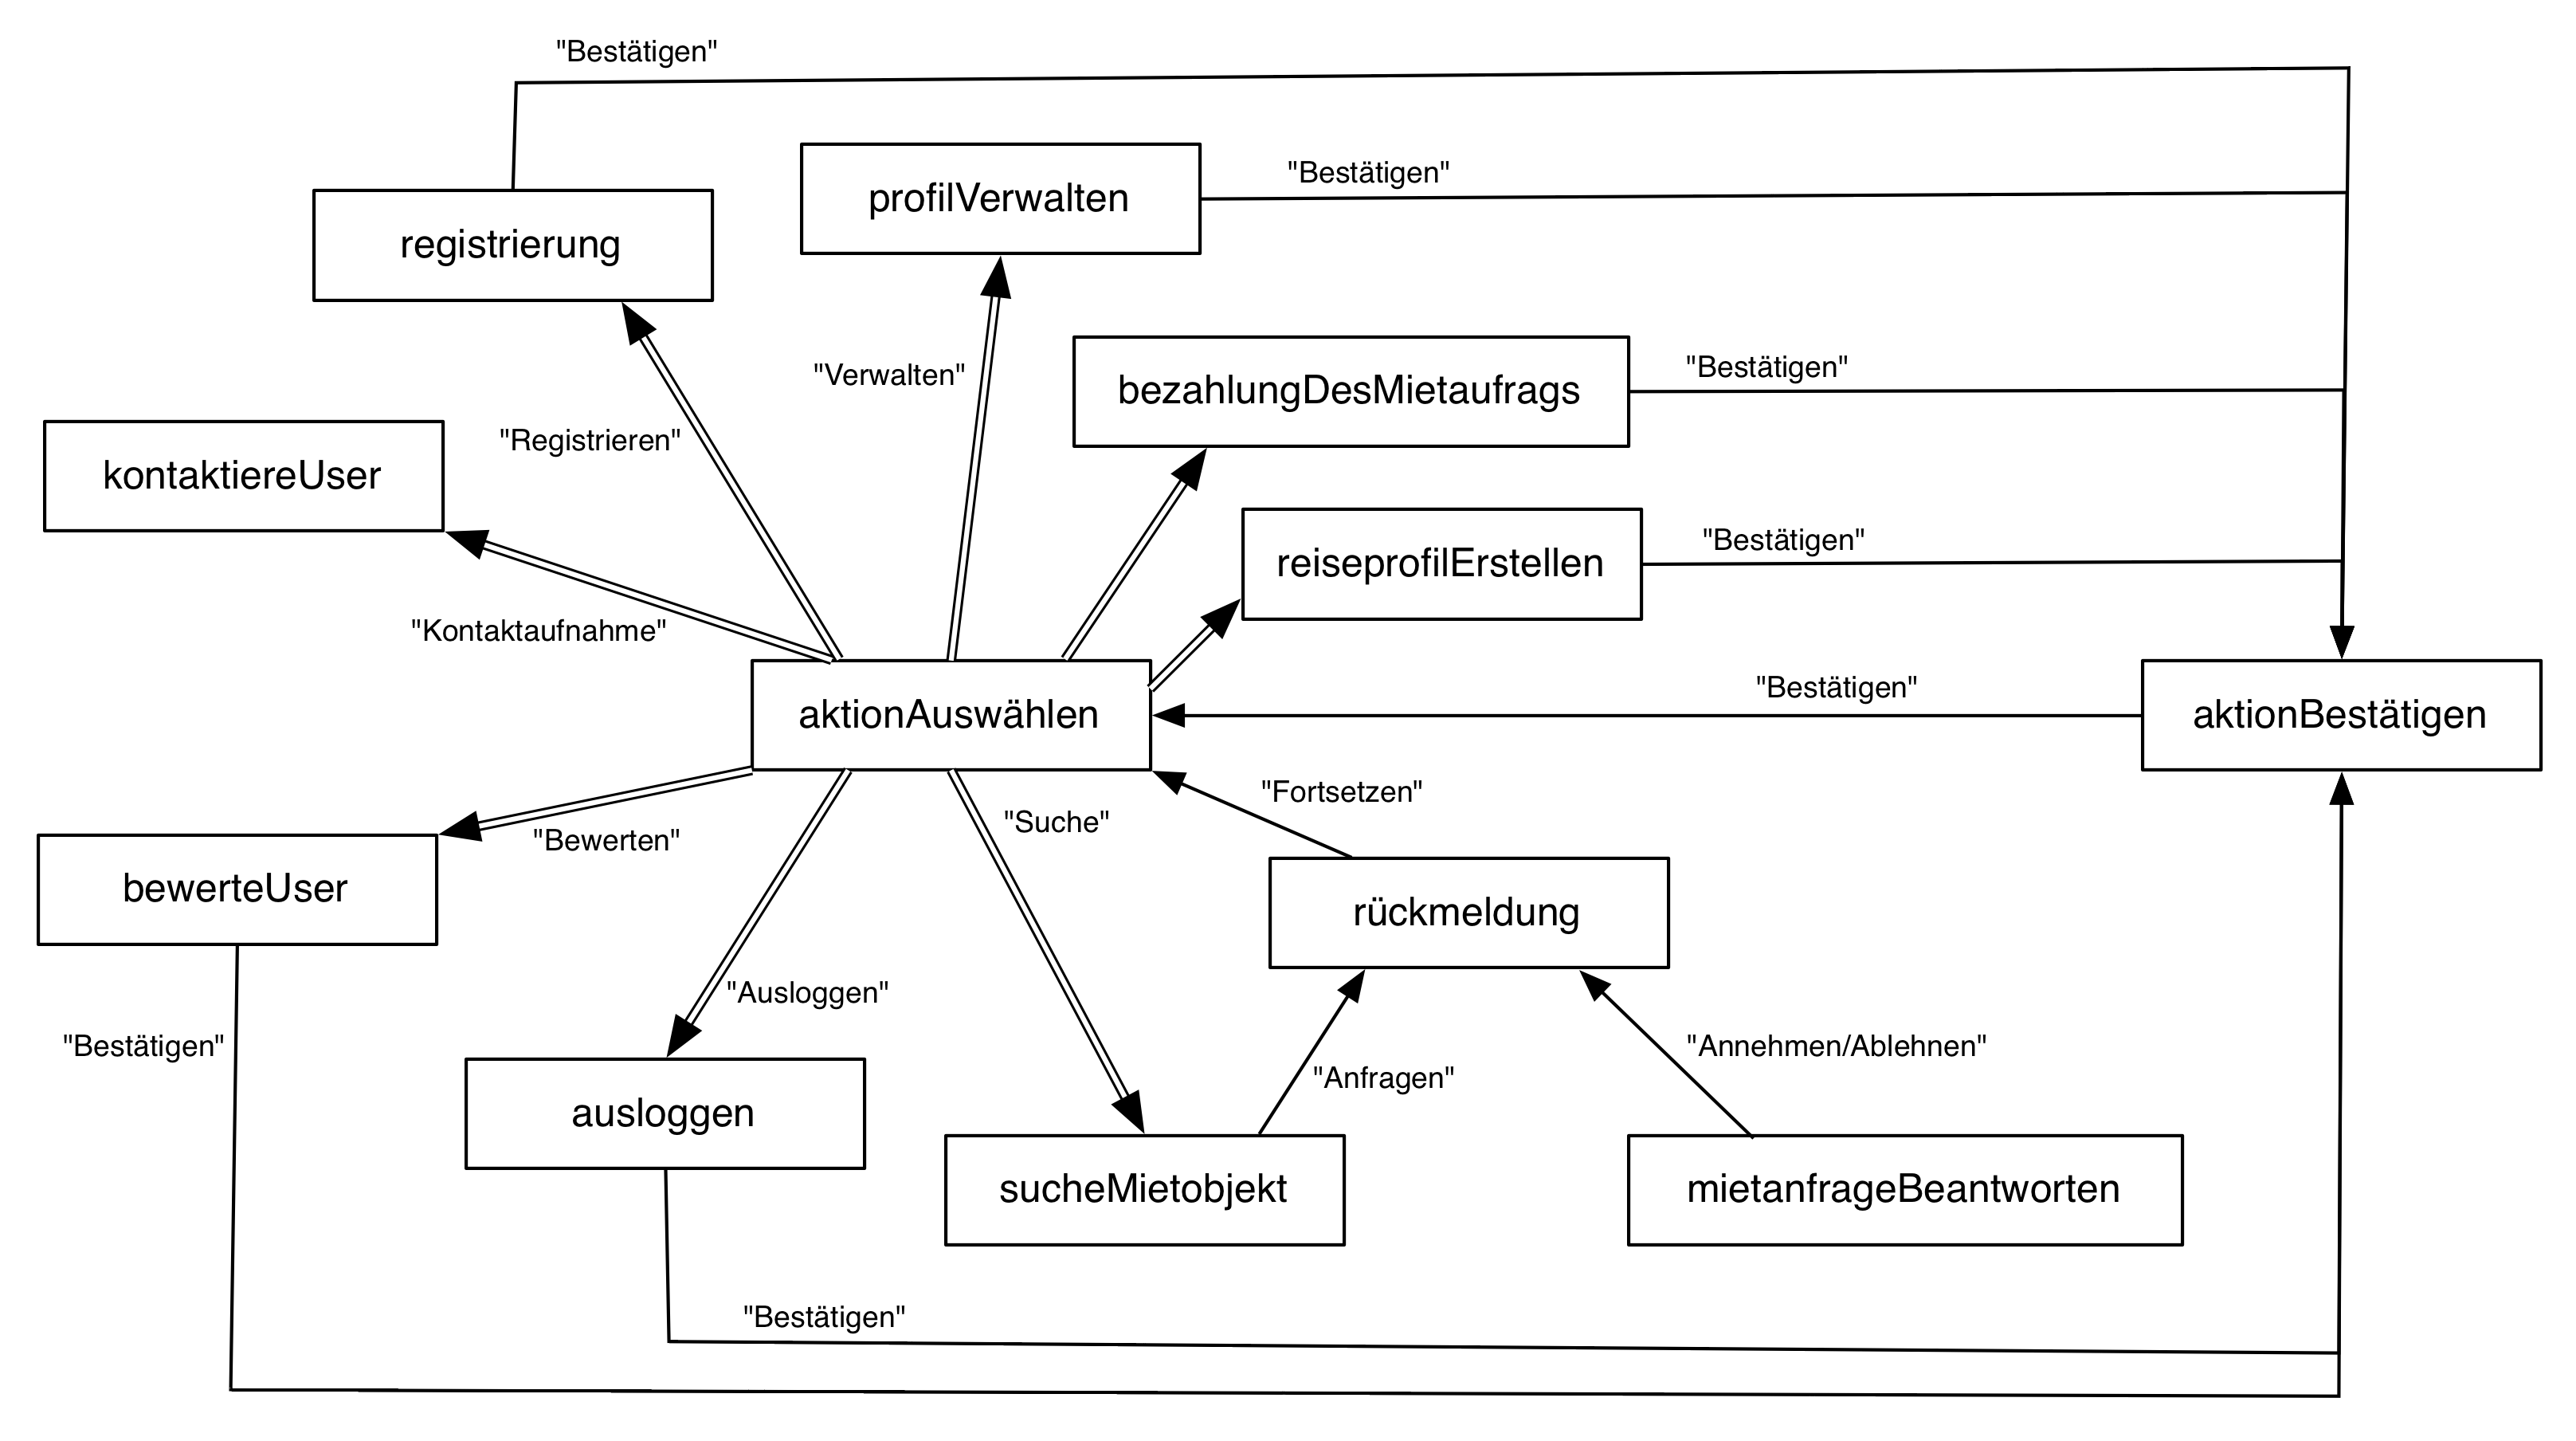
\includegraphics[width=1\textwidth]{./images/navigationmap1.png}
\caption{Context Navigation Map Version 1}
\label{fig:navigationmap1}
\end{figure}

\subsubsection{Evaluation}
Mit dieser Navigation Map fand innerhalb des Projektteams eine erste Evaluation der Interface Architektur statt. Mit einer, an das cognitive walkthrough erinnernde Methode, wurden verschiedene Anwendungsfälle durchgespielt und dabei mit einfachen Mockups visualisiert. Dabei wurde ermittelt, dass es die zuvor entwickelte use case map deutlicher mit einbezogen werden sollte. Speziell durch den Anwendungsfall "aktionAuswählen", ergab sich eine Interfacestruktur, die von einem zentralen Working Space ausging und keine direkten Bezüge zwischen use cases darstellt, die eigentlich im direkten Zusammenhang stehen sollten. Wie beispielsweise, dass sowohl die Bezahlung, Bewertung und Kontaktaufnahme an einen einzelnen Mietauftrag gebunden sind.\\

\newpage
\subsection{Abstract Prototype 2}
Im Anschluss an die Evaluation des ersten Abstract Prototype (Kapitel 2.4.1), wurde es als notwendig erachtet, die bisherigen Ergebnisse in einer Iteration zu überarbeiten. Bereits während der vorherigen Kapitel wurde erwähnt, dass die einzelnen Abschnitte nicht zeitlich aufeinander folgend entstanden sind. \\
Um ein besseres Verständnis zum Projektverlauf bis an diesem Punkt zu vermitteln, zeigt die Abbildung \ref{fig:navigationmap3}, welche MCI Auseinandersetzung stattfanden, um an den derzeitigen Punkte der Prozessdokumentation anzugelangen.

\begin{figure}[H]
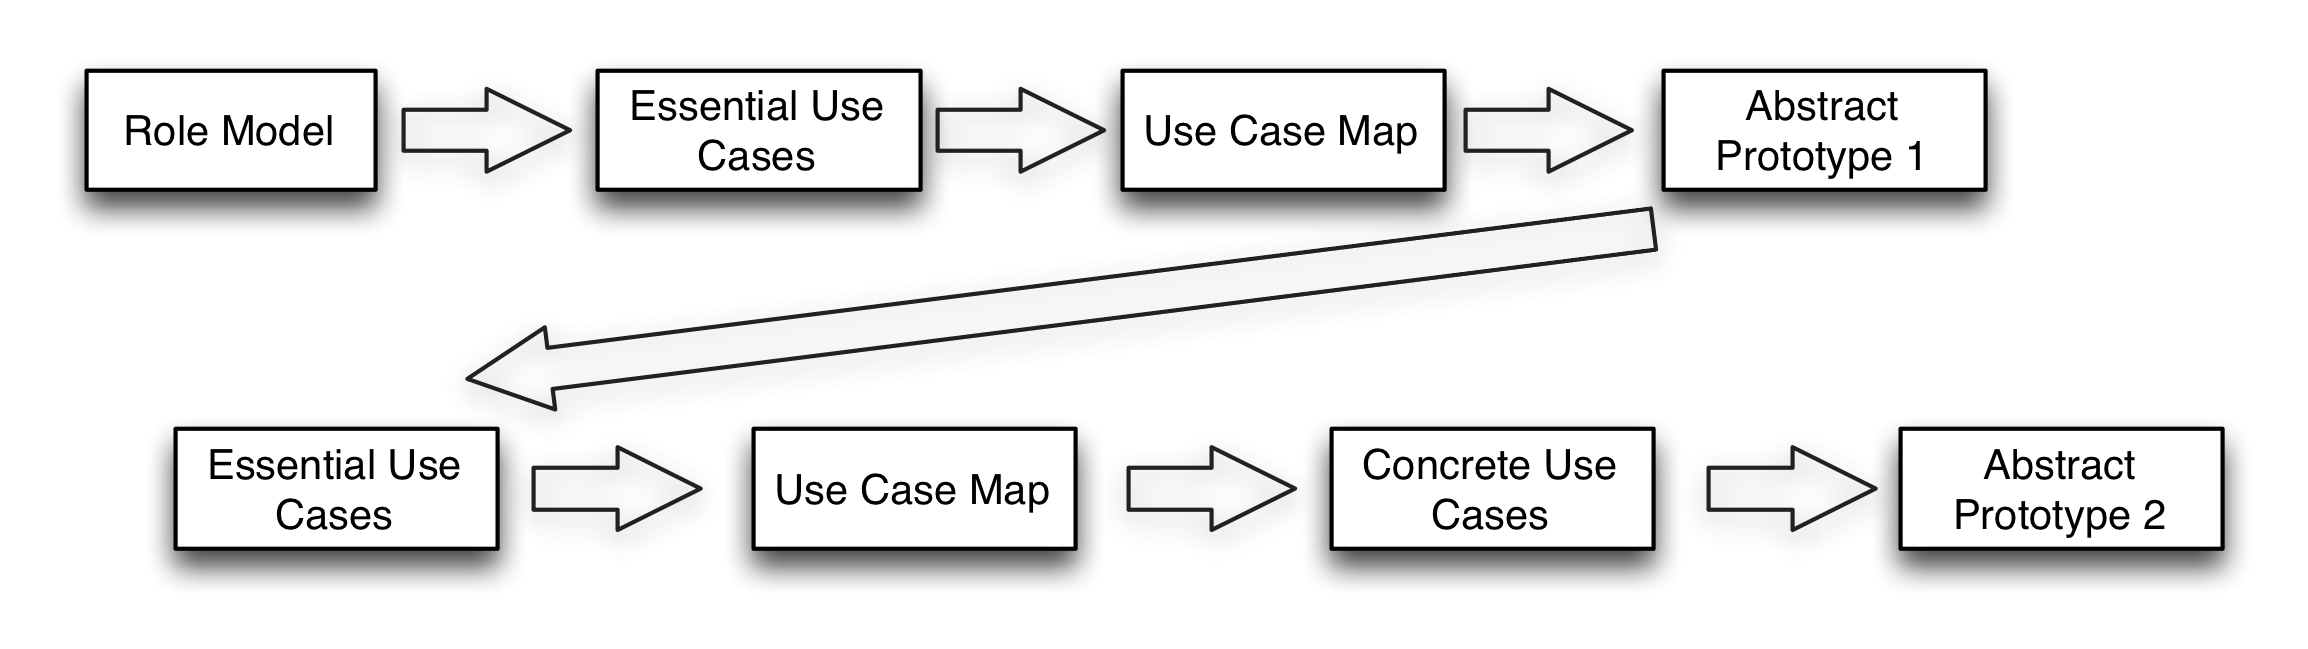
\includegraphics[width=1\textwidth]{./images/position.png}
\caption{Projektverlauf bis zu diesem Dokumentationspunkt}
\label{fig:navigationmap3}
\end{figure}

Die Aufgabenmodellierung wurde demnach einer kompletten Überarbeitung unterzogen und lieferte die Ergebnisse die im Vorfeld dargelegt waren. Anschließend folgte die zweite Version des Abstract Prototype.

\newpage
\subsubsection{Interaction Contexts }
Nach ähnlichem Prinzip wie im ersten Anlauf, wurden anhand der essentiell use cases interaction contexts erarbeitet. Abbildung \ref{interfaceContents2} zeigt dabei Entwürfe des zweiten Ansatzes.\footnote{Gesamtes Bilderset im Anhang Teil B}. Was sich am Vorgehen im Vergleich zur ersten Variante geändert hat, war unter anderem der Gestaltungsansatz. Orientiert am Format des Smartphonedisplays, wurden die neuen Seiten stärker mit Bezug zum Interface gestaltet. Auch wenn hierbei weiterhin ein minimalistischer Ansatz verfolgt wird, sollte die Positionierung der tools und materials einen ersten Aufwand über mögliche Plazierungen der Inhalte vermitteln. Vorteilhaft erwies sich hierbei der verstärkte Einbezug der Use Case Map, wobei zusätzlich angedachte Anwendungsfälle bereits mitverarbeitet wurden.

\begin{figure}[H]
\centering
\hfill
\subfloat[anzeigenVorhandenerAktionen \label{pic:anzeigenVorhandenerAktionen}]{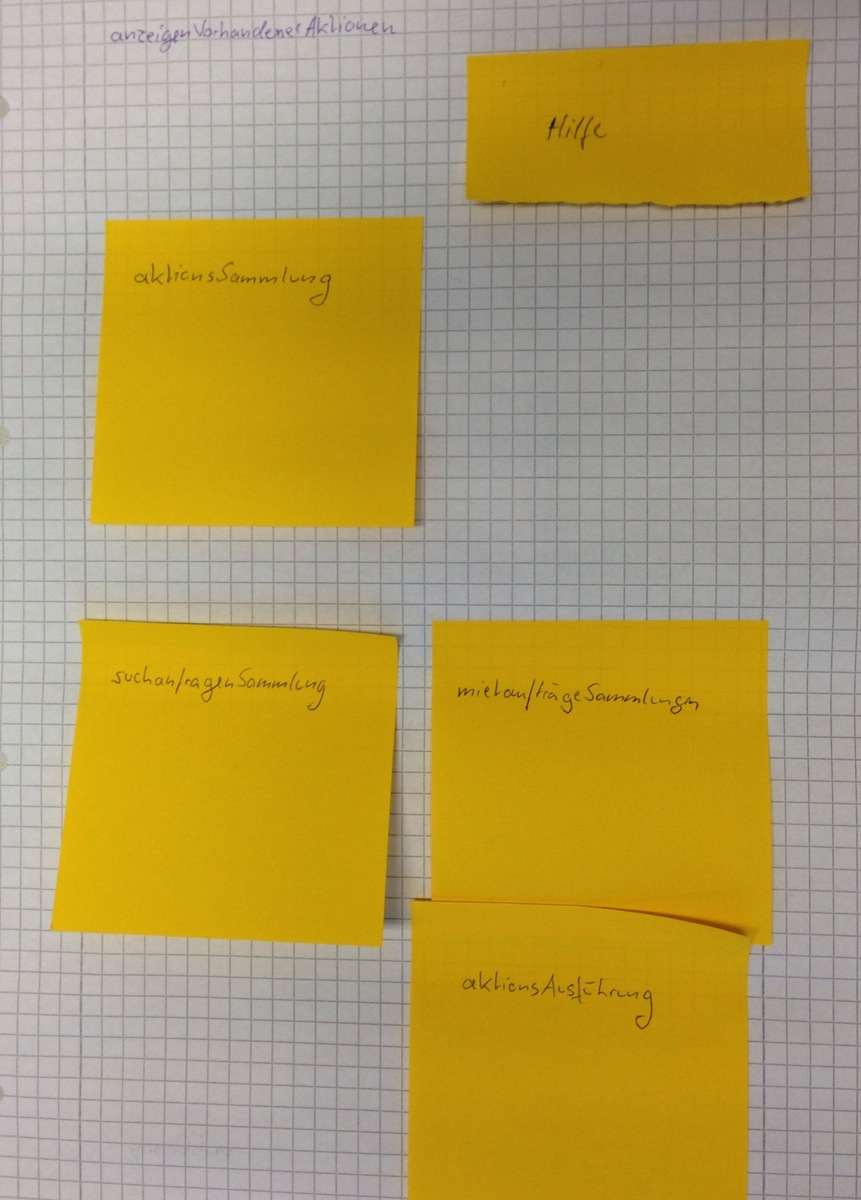
\includegraphics[width=.5\textwidth]{./images/abstract/version2/anzeigenVorhandenerAktionen.JPG}}
\hfill % alternativ auch \hspace{1cm} für genaue Angaben
\subfloat[suchanfrageStarten \label{pic:suchanfrageStarten}]{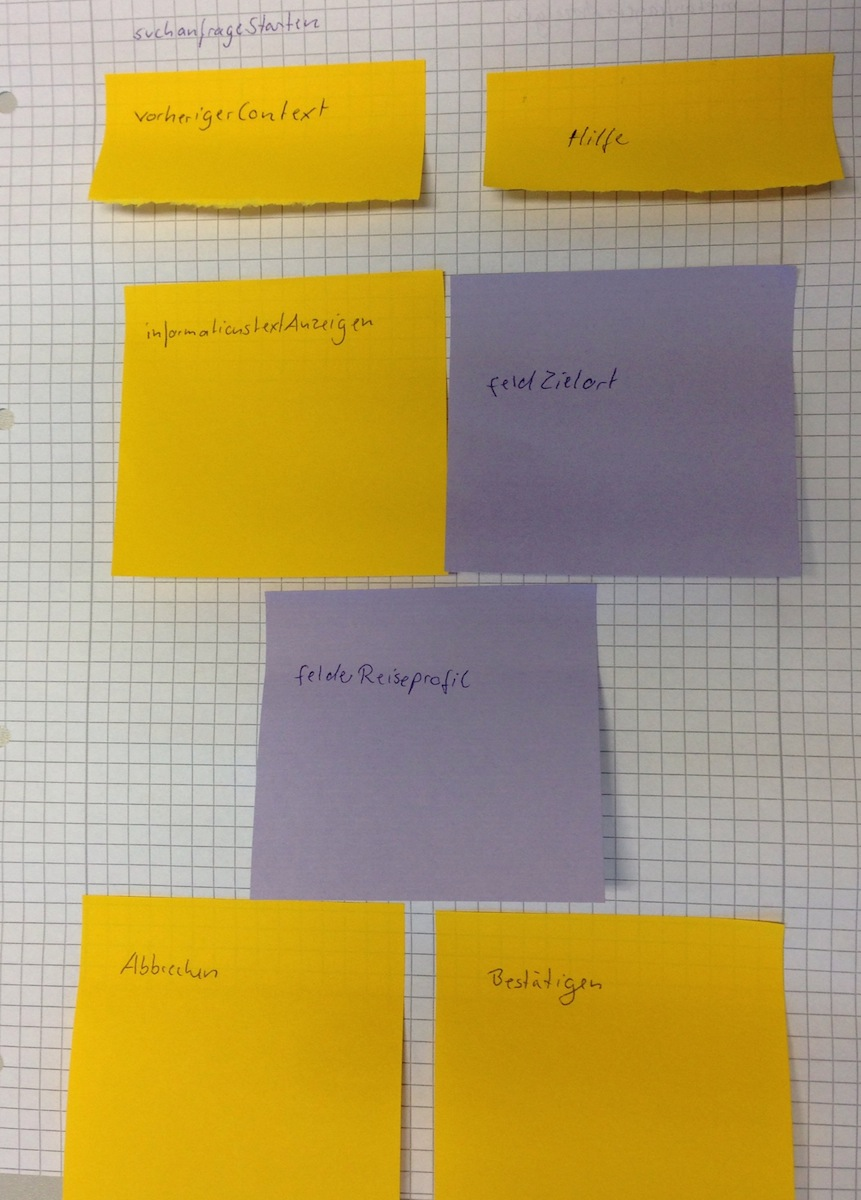
\includegraphics[width=.5\textwidth]{./images/abstract/version2/suchanfragenStarten.JPG}}
\hfill %
\caption{Inter. Context AP2: anzeigenVorhandenerAktionen und suchanfrageStarten }
\label{interfaceContents2}
\end{figure}

\newpage
\subsubsection{Context Navigation Map}
Aus den Ergebnissen wurde erneut eine Navigation Map, zu sehen in Abbildung \ref{fig:navigationmap2}, abgleitet und diesmal mit angemessener Notation dargestellt.
\begin{figure}[H]
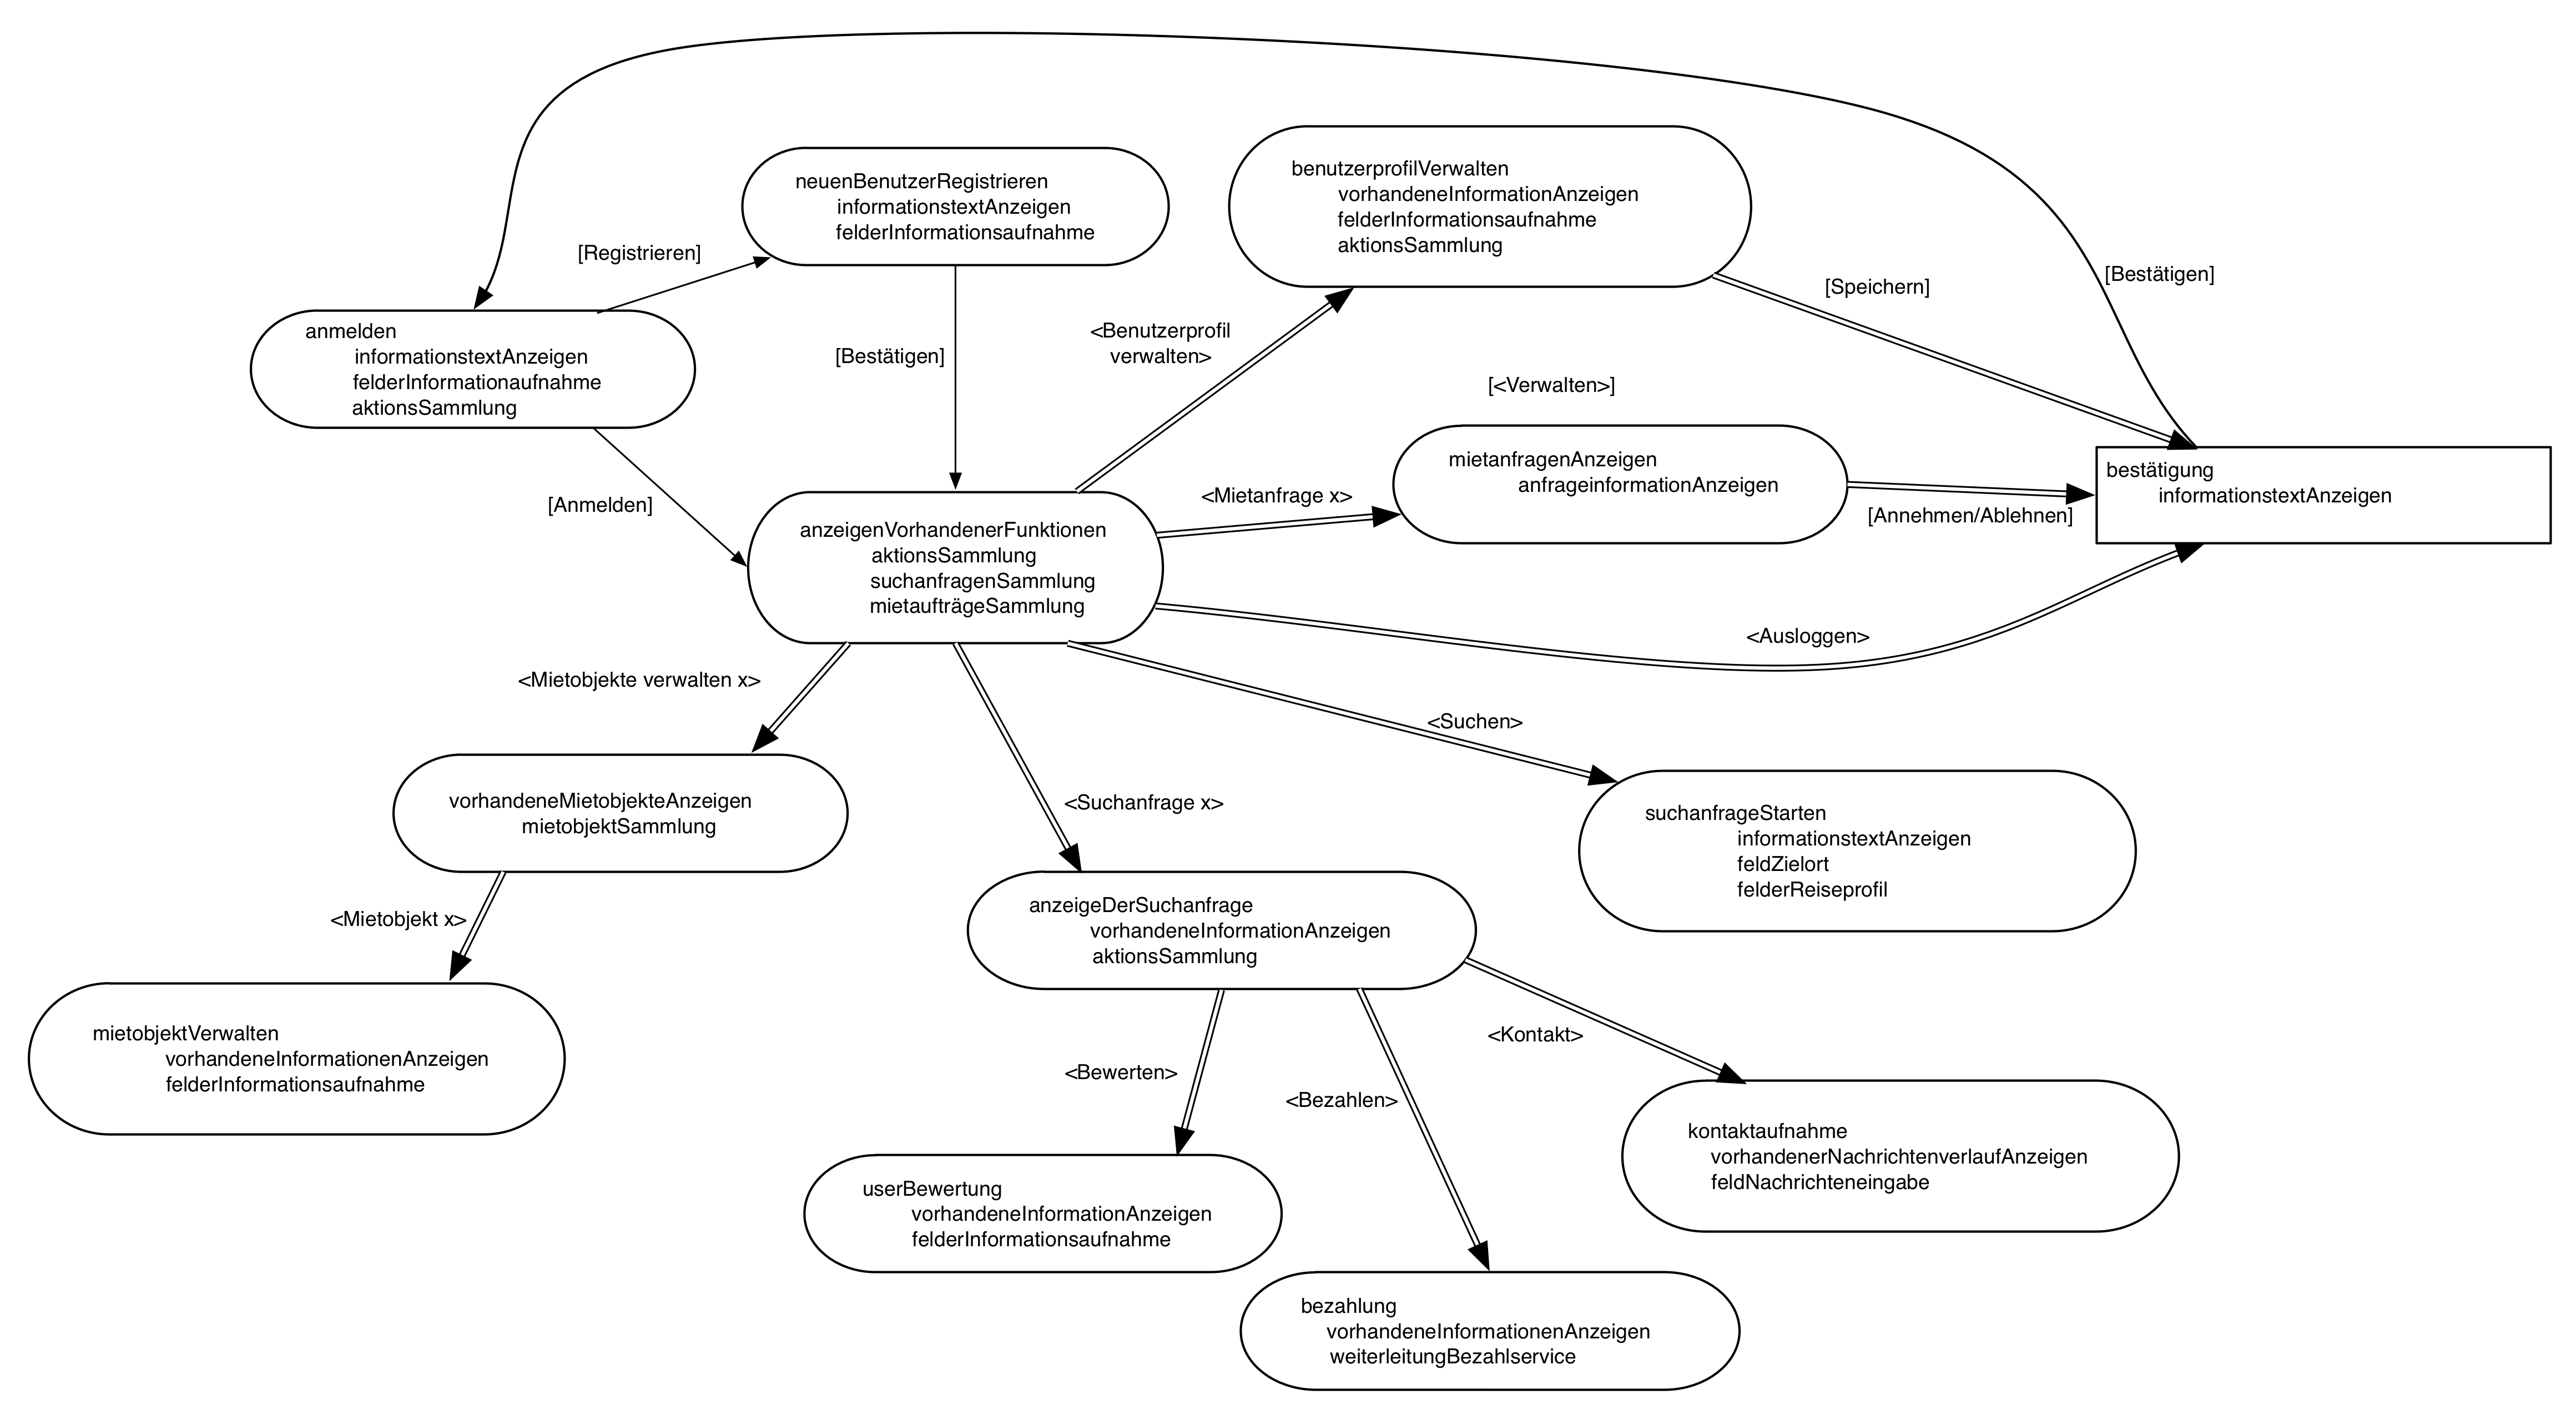
\includegraphics[width=1\textwidth]{./images/navigationmap2.png}
\caption{Context Navigation Map Version 2}
\label{fig:navigationmap2}
\end{figure}

Die Version 2 der Navigation Map, und somit das Content Model, wurden einer erneuten Evaluation unterzogen, bei der verschiedene Anwendungsfälle gedanklich durchgespielt wurden. Im Vergleich zum ersten Prototyp zeigte sich hierbei eine stark verbesserte Struktur, die den Aufgabenfluss im Gegensatz zur ersten Variante deutlich optimiert. Die erneute Auseinandersetzung führte im Projektverlauf dazu, dass Gestaltungslösungen erst später betrachtet wurden als ursprünglich geplant, jedoch lieferte das überarbeitete Content Model eine bedeutend bessere Vorlage.



